% main.tex -- paper draft. Build: see README.md in this folder (latexmk -pdf main.tex).
% Sections live in sections/*.tex so that each part can be edited independently.
\documentclass[11pt]{article}

\usepackage[utf8]{inputenc}
\usepackage[T1]{fontenc}
\usepackage{lmodern}
\usepackage[a4paper,margin=1in]{geometry}
\usepackage{amsmath,amssymb,amsthm}
\usepackage{mathtools}
\usepackage{bm}
\usepackage{booktabs}
\usepackage{multirow}
\usepackage{array}
\usepackage{graphicx}
\usepackage{xcolor}
\usepackage{microtype}
\usepackage[numbers,sort&compress]{natbib}
\usepackage[hidelinks]{hyperref}
\usepackage[capitalise,noabbrev]{cleveref}

% Figures are shared with the repository docs; make_arxiv.sh flattens this for arXiv.
\graphicspath{{../img/}}

% ---------------------------------------------------------------- editing macros
% \todo{...}   something still to write or decide (red, visible in the PDF)
% \pending{...} a result that depends on an experiment that has not run yet (orange)
% Set \finaltrue to hide both before submission; the build then fails loudly if any remain
% (see README.md, "Before submitting").
\newif\iffinal
\finalfalse
\iffinal
  \newcommand{\todo}[1]{\errmessage{Unresolved TODO: #1}}
  \newcommand{\pending}[1]{\errmessage{Unresolved PENDING: #1}}
\else
  \newcommand{\todo}[1]{\textcolor{red}{[TODO: #1]}}
  \newcommand{\pending}[1]{\textcolor{orange}{[PENDING: #1]}}
\fi

% ---------------------------------------------------------------- notation
\newcommand{\X}{X}                          % source video
\newcommand{\U}{U}                          % uploaded video
\newcommand{\Y}{Y}                          % playback seen by a viewer
\newcommand{\Gt}{G_{\theta}}                % pre-compensation
\newcommand{\fp}{f}                         % platform black box
\newcommand{\Em}{E_{\psi}}                  % learned emulator of f
\newcommand{\E}{\mathbb{E}}
\newcommand{\R}{\mathbb{R}}
\newcommand{\sg}{\operatorname{sg}}         % stop-gradient
\DeclareMathOperator*{\argmax}{arg\,max}
\newtheorem{definition}{Definition}
\newtheorem{proposition}{Proposition}
\newtheorem{remark}{Remark}

\title{Does Pre-Compensation Help Beyond the Resolution Tier Trick?\\
\large A Pre-Registered Study of Uploader-Side Optimisation Against Black-Box Video Platforms}
\author{{Haoran Zhao} \\ {The Ohio State University} \\ {zhao.4887@osu.edu}}
\date{{\today}}

\begin{document}
\maketitle

% Abstract. arXiv's abstract field is plain text and limited to 1920 characters; keep this in sync
% with what you paste into the submission form (no LaTeX commands, no citations there).
\begin{abstract}
Video platforms re-encode every upload with a policy the uploader cannot observe: the codec, bit
budget and ingest filtering depend on properties of the upload itself. A common creator heuristic
exploits this by uploading at a higher resolution to obtain a better encoding tier. We ask whether
an uploader can recover quality \emph{beyond} this tier trick by optimising a pre-compensation
applied before upload, treating the platform as a non-differentiable black box. We study two
routes, sample-efficient black-box search over an interpretable filter chain and a learned
pre-compensation network trained through a differentiable emulator of the platform, and we
separate the tier gain from the filter gain. On simulated platforms, the optimised pre-compensation
improves the training objective by a large margin, but independent metrics that were not optimised
(SSIMULACRA2, XPSNR, DISTS) confirm only the tier gain; most of the apparent filter gain is colour
and contrast change that the objective rewards. Every single-metric objective we tried degrades at
least one metric it did not optimise. A learned pre-compensation exploits its emulator unless it is
constrained by a trust region. In a pre-registered design with held-out confirmation clips, a
learned pre-compensation does not beat class-tuned sharpening on natural low-motion content.
Anchoring its forward pass on the black box closes about 80\,\% of the gap, showing emulator
exploitation; the rest trades the independent metrics for its training loss. An untuned mild
sharpening applied only to natural low-motion content matches the tuned configuration, and the
upload bitrate matters more than any filter. The benefit depends on the platform's rate headroom;
validating it on a platform takes about 20 uploads.
\pending{P2 result: real-platform validation and viewer study.}
Code, clip manifests and the pre-registration are released.
\end{abstract}

\section{Introduction}
\label{sec:intro}

User-generated video reaches its viewers only after the hosting platform has re-encoded it. The
platform decides, from properties of the upload that the uploader controls only indirectly, which
codec, which rate-control target and which ingest filtering to apply, and which rendition each
viewer receives~\cite{meta2021facebook}. None of these decisions is documented, and none can be
differentiated through. As a consequence, uploading the best possible master is not the same as
delivering the best possible playback.

Creators have developed heuristics for this situation. The best known is the \emph{tier trick}:
upscaling a 1080p video to 1440p or 4K before upload so that the platform assigns a more efficient
codec and a larger bit budget. Whether anything beyond this heuristic is available to an uploader
is an open question. Encoder-side pre-processing is well studied: learned pre-processors in front of
standard encoders reduce bitrate at equal quality~\cite{bourtsoulatze2020deep,chadha2021deep,
ma2023rate,zhao2025tridynamic}. These methods, however, are deployed by the party that runs the
encoder and knows its settings. The uploader faces a different problem: the encoder, its settings
and the ladder that selects them are hidden, and every evaluation costs a real upload.

\paragraph{This paper.}
We formulate uploader-side pre-compensation as black-box optimisation of a transform
$\Gt$ applied before upload, so that the playback $\Y = \fp(\Gt(\X))$ is close to the source
$\X$ (\cref{sec:problem}). We study two routes: sample-efficient search over an interpretable
seven-parameter filter chain, and a learned residual network trained through a differentiable
emulator of the platform (\cref{sec:method}). Our evaluation is designed around two pitfalls that we
found to dominate the outcome:
\begin{enumerate}
  \item \textbf{Tier gain versus filter gain.} Most of the improvement comes from selecting a
        better encoding tier. We decompose every result into the tier gain and the filter gain on
        top of it.
  \item \textbf{Objective versus judge.} An optimiser finds whatever its objective rewards. We
        separate the optimised metric from independent judge metrics, and we count a gain only if
        the judges agree~\cite{zvezdakova2019hacking,siniukov2021hacking}.
\end{enumerate}

\paragraph{Contributions.}
\begin{itemize}
  \item A formulation of uploader-side pre-compensation against an adaptive, non-differentiable
        platform pipeline, with a decomposition of the gain into a tier component and a filter
        component (\cref{sec:problem}).
  \item Evidence, on simulated platforms, that the filter gain found by optimising a composite of
        VMAF NEG, LPIPS and CAMBI is not confirmed by SSIMULACRA2 and XPSNR, and that every
        single-metric objective degrades at least one judge it does not optimise (a ``Goodhart
        matrix'', \cref{sec:results-p0}).
  \item A documented failure mode of emulator-based training (exploitation of the emulator) and its
        mitigation by a trust region (\cref{sec:results-p0}).
  \item A pre-registered, content-scoped test of a learned pre-compensation with a content gate,
        evaluated once on held-out confirmation clips (\cref{sec:results-p1}).
        \pending{state the outcome.}
  \item \pending{Real-platform measurements: ladder probe, closed loop and viewer study
        (\cref{sec:results-p2}).}
  \item An open-source implementation, clip manifests with per-clip licenses, and the
        pre-registration files.
\end{itemize}

\section{Related Work}
\label{sec:related}
% Sources: docs/related-work.md. Every claim here must be checked against the cited paper itself
% before submission; several entries in references.bib are still marked "unverified".

\paragraph{Learned pre-processing for standard codecs.}
Deep video precoding~\cite{bourtsoulatze2020deep} and deep perceptual
preprocessing~\cite{chadha2021deep} place a neural network in front of AVC, HEVC, VP9, AV1 or VVC
encoders and train it through a differentiable proxy of the codec; the decoder is unchanged.
Rate-perception optimised preprocessing~\cite{ma2023rate} is reported to run in a production
transcoding service. For user-generated content, a deep pre-processor tuned on pristine data was
found to make a substantial fraction of clips worse, which motivated adaptive control of the
pre-processing strength~\cite{zhao2025tridynamic}. Pre-editing before JPEG with a learned network
is the image analogue~\cite{talebi2021better}. All of these methods are applied by the party that
runs the encoder. Our setting differs in that the encoder, its configuration and the ladder that
chooses it are unknown to the optimiser. \todo{check each paper's exact setting and numbers.}

\paragraph{Training through non-differentiable codecs.}
Codec surrogates replace the real codec by a network during
training~\cite{tian2021self,chadha2021deep}. Alternatively, the real codec can be run in the
forward pass while a surrogate supplies the gradient~\cite{pesnel2026scaled}, an instance of the
straight-through and backward-pass-approximation
idea~\cite{bengio2013estimating,athalye2018obfuscated}. Accurate differentiable approximations exist
for simple codecs such as JPEG~\cite{reich2024differentiable}. Our emulator is a surrogate of the
entire platform pipeline rather than of a single codec.

\paragraph{Optimising against learned models.}
Optimising against a learned model drives the optimiser towards inputs on which the model
overestimates the objective. Offline model-based optimisation counters this with conservative
objective models~\cite{trabucco2021conservative}; model-based reinforcement learning penalises
ensemble disagreement~\cite{yu2020mopo}; trust-region Bayesian optimisation restricts the search
locally~\cite{eriksson2019scalable}. We observe the same failure when training a pre-compensation
through a platform emulator.

\paragraph{Metric hacking.}
VMAF~\cite{li2016toward} can be raised substantially by sharpening and by colour and contrast
changes without a subjective improvement~\cite{zvezdakova2019hacking}; the NEG variant reduces but
does not remove this~\cite{siniukov2021hacking,fingscheidt2026optimizing}. This is an instance of
Goodhart's law~\cite{manheim2018categorizing}. Our evaluation therefore separates the optimised
objective from judge metrics, following the recommendation to verify with metrics that were not
optimised.

\paragraph{Closed-loop adaptation to real platforms.}
Robust steganography uses transport channel matching: an image is uploaded to a social network
repeatedly until recompression no longer changes it~\cite{zhao2019improving}. This is the closest
methodological precedent for a closed loop against a real platform, with a different goal. Work on
the quality of user-generated content notes that the platform's reference is itself already
distorted~\cite{yu2021predicting,wang2019youtube}.

\paragraph{Black-box optimisation.}
We use Gaussian-process Bayesian optimisation~\cite{snoek2012practical,shahriari2016taking}, the
tree-structured Parzen estimator~\cite{bergstra2011algorithms}, CMA-ES~\cite{hansen2001completely}
and random search as implemented in Optuna~\cite{akiba2019optuna}.

\section{Problem Formulation}
\label{sec:problem}

\subsection{The platform as a black-box channel}

Let $\X$ be a source video. The uploader applies a pre-compensation $\Gt$ with parameters
$\theta\in\Theta$ and uploads $\U=\Gt(\X)$. The platform returns the playback that a viewer receives,
\begin{equation}
  \Y = \fp(\U) = R \circ C_{\tau(\U)} \circ D_{\tau(\U)}(\U),
  \label{eq:platform}
\end{equation}
where $\tau(\U)$ is the \emph{ladder policy} that selects a tier from observable properties of the
upload (resolution, bitrate, possibly content and popularity), $D_\tau$ is the tier's ingest
filtering (e.g.\ denoising), $C_\tau$ is the tier's encoder with its rate control, and $R$ resamples
to the rendition served to the viewer. The uploader can only query $\fp$; $\tau$, $D$ and $C$ are
unknown, $\tau$ is piecewise constant, and $C$ includes quantisation, so $\fp$ is neither known nor
differentiable. Each query costs a real upload.

Playback quality is measured against the source with a full-reference metric $M(\Y,\X)$ (higher is
better), after resampling $\Y$ to the resolution of $\X$. The uploader's problem is
\begin{equation}
  \theta^\star = \argmax_{\theta\in\Theta}\; J_M(\theta),\qquad
  J_M(\theta) = \E_{\X\sim\mathcal{D}}\big[M\big(\fp(\Gt(\X)),\X\big)\big],
  \label{eq:objective}
\end{equation}
over a distribution $\mathcal{D}$ of source videos. In practice the expectation is an average over a
finite set of clips.

\subsection{Tier gain and filter gain}

We split the parameters into a \emph{tier} component $s$ (here the upload scale factor, which
changes $\tau(\U)$) and a \emph{filter} component $\varphi$ (sharpening, grain, colour, denoising),
$\theta=(s,\varphi)$, with identities $s_0$ (no rescaling) and $\varphi_0$ (no filtering).

\begin{definition}[Gain decomposition]
\label{def:decomposition}
For parameters $\theta=(s,\varphi)$, the total gain over a naive upload splits as
\begin{equation}
  \underbrace{J_M(s,\varphi)-J_M(s_0,\varphi_0)}_{\text{total gain}}
  = \underbrace{J_M(s,\varphi_0)-J_M(s_0,\varphi_0)}_{\text{tier gain}}
  + \underbrace{J_M(s,\varphi)-J_M(s,\varphi_0)}_{\text{filter gain at tier } s}.
  \label{eq:decomposition}
\end{equation}
\end{definition}

The split is exact, but it depends on the order: the filter gain at tier $s$ generally differs from
the filter gain at $s_0$, because the filter interacts with the tier's encoder and ingest filtering.
We report the tier-first order, since the tier is discrete and its effect is large, and we measure
the filter gain at the native tier separately (\cref{sec:results-p0}). A pre-compensation is useful
beyond the creator heuristic only if its filter gain is positive.

\subsection{Objectives, judges and Goodhart's law}
\label{sec:goodhart}

The metric $M$ is a model of perceived quality $Q$. Write $M = Q + \varepsilon$, where
$\varepsilon(\theta)$ is the metric's error at the playback produced by $\theta$. The following
statement is a version of the optimiser's curse~\cite{smith2006optimizer}; we state it because it
explains why the gains we report on the optimised metric are biased upwards.

\begin{proposition}[Selection inflates the optimised metric]
\label{prop:curse}
Let $\Theta_n\subset\Theta$ be the finite set of candidates evaluated by a search, let
$\hat\theta=\argmax_{\theta\in\Theta_n} J_M(\theta)$, and let
$\theta^\dagger=\argmax_{\theta\in\Theta_n} J_Q(\theta)$ be the truly best candidate. If the metric
error has zero mean at $\theta^\dagger$, $\E[\varepsilon(\theta^\dagger)]=0$ (for instance, because
the error is independent of $Q$ and unbiased at every fixed $\theta$), then
\begin{equation}
  \E\big[\varepsilon(\hat\theta)\big] \;\ge\; \E\big[J_Q(\theta^\dagger)-J_Q(\hat\theta)\big] \;\ge\; 0 .
\end{equation}
\end{proposition}

\begin{proof}
By the definition of $\hat\theta$, $J_Q(\hat\theta)+\varepsilon(\hat\theta) \ge
J_Q(\theta^\dagger)+\varepsilon(\theta^\dagger)$, hence $\varepsilon(\hat\theta) \ge
\varepsilon(\theta^\dagger) + J_Q(\theta^\dagger)-J_Q(\hat\theta)$. Take expectations; the last
difference is non-negative by the definition of $\theta^\dagger$.
\end{proof}

The proposition covers errors that are noise-like. A more harmful case is an error with structure:
if $\varepsilon$ grows along some direction of $\Theta$ (for example, a metric that rewards a
contrast increase), the optimiser moves along that direction and the inflation is no longer bounded
by the noise level. This is the regime documented for VMAF and VMAF
NEG~\cite{zvezdakova2019hacking,siniukov2021hacking}.

We therefore distinguish the \emph{objective} $M$ from a set of \emph{judges}
$\mathcal{J}=\{M_1,\dots,M_K\}$, metrics that the optimiser never sees.

\begin{definition}[Judge-confirmed gain]
\label{def:confirmed}
A gain of configuration $a$ over configuration $b$ is \emph{judge-confirmed} if at least $k$ of the
$K$ judges assign $a$ a higher mean score than $b$ over the evaluation clips. In P0 we use $K=3$ and
$k=2$; in P1 we additionally require a confidence interval over clips that excludes zero
(\cref{sec:decision}).
\end{definition}

\begin{remark}
If the judges' errors were independent of each other and of the objective's error, the probability
that a gain which is spurious for $Q$ appears on $k$ of $K$ judges would shrink geometrically in
$k$. Real metrics share failure modes (several react to sharpness or contrast in the same way), so
agreement among judges is evidence, not proof; a viewer study remains the final arbiter.
\end{remark}

\subsection{Optimising through a learned emulator}
\label{sec:emulator-theory}

For a learned pre-compensation, $\Gt$ is a network with millions of parameters, too many for
black-box search. We fit an emulator $\Em\approx\fp$ on pairs $\{(\U_i,\fp(\U_i))\}$ collected from the
black box, and train $\Gt$ by gradient ascent on the emulated objective
\begin{equation}
  J_M^{E}(\theta)=\E_{\X}\big[M\big(\Em(\Gt(\X)),\X\big)\big].
\end{equation}
If $M$ is $L$-Lipschitz in its first argument (with respect to a norm $\|\cdot\|$), then
\begin{equation}
  J_M(\theta) \;\ge\; J_M^{E}(\theta) - L\,\E_{\X}\big\|\fp(\Gt(\X))-\Em(\Gt(\X))\big\|.
  \label{eq:emulator-bound}
\end{equation}
The emulator error in the last term is small only on the distribution of uploads that $\Em$ was
trained on. Gradient ascent on $J_M^E$ moves $\Gt(\X)$ away from that distribution, towards inputs
where the emulator overestimates $M$, so the gap can grow without limit. This is the failure mode of
offline model-based optimisation~\cite{trabucco2021conservative,yu2020mopo}. We measure the gap
directly, by sending $\Gt(\X)$ through the real black box and reporting the emulator's PSNR against
the real playback, and we control it with a trust region:
\begin{equation}
  \min_\theta\; -J_M^{E}(\theta) + \lambda\,\E_{\X}\|\Gt(\X)-\X\|_1
  \quad\text{s.t.}\quad \|\Gt(\X)-\X\|_\infty\le\delta,
  \label{eq:trust}
\end{equation}
which keeps the uploads near the identity-like uploads in the emulator's training data.

A further option, not used in the experiments reported here, is a straight-through
estimator~\cite{bengio2013estimating,athalye2018obfuscated,pesnel2026scaled}: use the real playback
in the forward pass and the emulator only for the gradient,
\begin{equation}
  \tilde\Y = \fp(\U) + \Em(\U) - \sg\big(\Em(\U)\big),
\end{equation}
where $\sg$ is the stop-gradient operator. The objective's value is then always the real one, and
only its gradient is approximate.

\subsection{Content-scoped claims and gating}
\label{sec:content-theory}

The platform's damage depends systematically on content: rate control and ingest filtering respond
to texture, motion and flat regions. A pre-compensation that is not useful on average may still be
useful on a subset. Let $c(\X)$ be a class label computed from content features (\cref{sec:setup}),
with classes $k=1,\dots,K_c$ and class probabilities $p_k$, and let the class-conditional gain of
configuration $a$ over a baseline $b$ be
\begin{equation}
  \Delta_k(a,b)=\E\big[M(\fp(a(\X)),\X)-M(\fp(b(\X)),\X)\,\big|\,c(\X)=k\big].
\end{equation}
A \emph{gate} $\pi$ assigns one configuration to each class. Its gain over the baseline is
$\sum_k p_k\,\Delta_k(\pi(k),b)$, which is at least the gain of the best single configuration if
$\pi(k)$ is chosen per class with the true $\Delta_k$.

The difficulty is estimation. If the classes, the gate or the claim are chosen on the same clips
that are used to estimate $\Delta_k$, the estimate is inflated by selection, exactly as in
\cref{prop:curse}, with the choice of subgroup playing the role of the search. We therefore:
\begin{enumerate}
  \item define the classes from content features by a fixed rule, before any learned model is
        trained;
  \item split the clips into train, development and confirmation sets, grouped by source so that
        no source contributes to two splits;
  \item choose the gate and the claimed class on the development set only;
  \item evaluate the confirmation set once.
\end{enumerate}
This is a pre-registered design in the sense of~\cite{nosek2018preregistration}. The classes,
splits and decision rules are committed to the repository before training (\cref{sec:setup}).

\subsection{Decision rule}
\label{sec:decision}

The unit of analysis is the clip: seeds are averaged within a clip, and uncertainty is estimated
over clips with a percentile bootstrap~\cite{efron1993introduction} (10{,}000 resamples). For the
content-scoped hypothesis, a learned pre-compensation is said to help on class $k$ if, on the
confirmation clips of that class:
\begin{enumerate}
  \item at least two judges show a mean gain over the class-tuned sharpening baseline whose 95\%
        bootstrap interval excludes zero (97.5\% if a second class is tested);
  \item the mean SSIMULACRA2 gain is non-negative;
  \item the sign of the effect holds for at least two of three training seeds.
\end{enumerate}
A judge that is part of the network's training loss is not used to judge it.

\section{Method}
\label{sec:method}

\subsection{Parametric pre-compensation}
\label{sec:parametric}

The interpretable pre-compensation is a filter chain implemented with FFmpeg~\cite{ffmpeg}:
spatio-temporal denoising (\texttt{hqdn3d}), contrast and saturation (\texttt{eq}), Lanczos
upscaling, an unsharp mask on luma, and temporal luma grain. \Cref{tab:space} lists the seven
parameters. All are continuous; the upscale factor is snapped to $\{1, 1.5, 2\}$ and the unsharp
radius to $\{1,2,3\}$ (kernel size $3,5,7$), so the same space serves every sampler. The upscale
factor is the tier component $s$ of \cref{def:decomposition}; the other six form the filter
component $\varphi$. The upload is encoded near-losslessly (x264, CRF 10), so the uploader's own
compression is not a confounder.

\begin{table}[t]
  \centering
  \caption{Parameters of the interpretable pre-compensation. The identity value makes a step a
  no-op; trial 0 of every search is the identity (the naive upload).}
  \label{tab:space}
  \begin{tabular}{@{}llll@{}}
    \toprule
    Parameter & Range & Identity & Role \\
    \midrule
    denoise        & $[0, 6]$       & 0   & \texttt{hqdn3d} strength \\
    contrast       & $[0.90, 1.15]$ & 1   & \texttt{eq} contrast \\
    saturation     & $[0.85, 1.25]$ & 1   & \texttt{eq} saturation \\
    upscale        & $\{1, 1.5, 2\}$ & 1  & upload resolution factor (tier) \\
    sharpen        & $[0, 2]$       & 0   & unsharp amount on luma \\
    sharpen\_radius & $\{1, 2, 3\}$ & 1   & unsharp kernel $3\times3$, $5\times5$, $7\times7$ \\
    grain          & $[0, 15]$      & 0   & temporal luma noise (dither) \\
    \bottomrule
  \end{tabular}
\end{table}

\paragraph{Search.}
We compare Gaussian-process Bayesian optimisation (GP-BO, 8 start-up trials), multivariate
TPE (8 start-up trials), CMA-ES (population 8) and random search, all from
Optuna~\cite{akiba2019optuna}, with a budget of 40 trials. A trial renders the upload, sends it
through the platform and scores the playback on every clip of the training set; the objective is
the mean over clips. Evaluations are cached by $(\text{clip},\theta)$, so studies, transfers and
re-scoring share work.

\subsection{Learned pre-compensation through an emulator}
\label{sec:learned}

\paragraph{Networks.}
Both the emulator $\Em$ and the pre-compensation $\Gt$ are residual U-Nets~\cite{ronneberger2015unet}
of the form $y = x + r\tanh(h(x))$, with the last convolution initialised to zero so that each
network starts as the identity. The emulator has width 32, three levels and $r=1$. The
pre-compensation has width 24, two levels and a hard bound $r=\delta=0.06$ on its per-pixel change
(on a $[0,1]$ scale). Both operate on RGB frames; the upload tier is fixed at $\times 2$ for the
learned route, since the tier is settled by the parametric study.

\paragraph{Training.}
In round 0 we send, for each training clip, the identity and five random parametric
pre-compensations (at the source resolution) through the black box, and keep every fourth frame of
each (upload, playback) pair. The emulator is trained with an $\ell_1$ loss on aligned
$256\times256$ crops (AdamW, 3000 steps). The pre-compensation is then trained through the frozen
emulator with
\begin{equation}
  \mathcal{L}(\theta) = \mathrm{LPIPS}\big(\Em(\Gt(x)), x\big)
  + \big\|\Em(\Gt(x)) - x\big\|_1
  + \lambda\,\big\|\Gt(x) - x\big\|_1,
  \label{eq:gloss}
\end{equation}
with LPIPS (AlexNet)~\cite{zhang2018unreasonable}, $\lambda=2$ (the trust region of
\cref{eq:trust}) and 1500 Adam steps. In P1 the perceptual term can also be
DISTS~\cite{ding2022image} or the sum of both. After each round, $\Gt$'s outputs are sent through the
real black box; their real playback is added to the emulator's data for the next round (domain
adaptation), and the emulator's PSNR against the real playback is logged as the measured
sim-to-real gap.

\paragraph{Real-anchored estimator.}
\label{sec:anchored}
To test whether $\Gt$ fails because it exploits the emulator (\cref{sec:emulator-theory}), we also
train it with a forward value anchored on the black box. Training is split into $A$ phases. At the
start of phase $k$, the current $G_k$ is applied to every training clip and sent once through the
black box, giving $y^{\text{real}}_k=\fp(G_k(x))$, and the offset
$\Delta_k = y^{\text{real}}_k - \Em(G_k(x))$ is stored. During the phase the loss of \cref{eq:gloss}
is evaluated on
\begin{equation}
  \hat y = \Em(\Gt(x)) + \sg(\Delta_k),
  \label{eq:anchored}
\end{equation}
which equals the black box's output at the anchor, adds the emulator's predicted change away from
it, and back-propagates the emulator's gradient. This is the straight-through estimator
$y^{\text{real}} + \Em(x) - \sg(\Em(x))$~\cite{bengio2013estimating,tian2021self,pesnel2026scaled} with the real output refreshed once per
phase; a per-step refresh would cost one upload per clip and step. Each anchor costs one black-box
call per training clip.

\paragraph{Pre-compensation on top of a tuned configuration.}
To ask whether $\Gt$ can add to a tuned interpretable configuration $\theta^\ast$ rather than compete
with it, we move $\theta^\ast$ into the channel: the upload is $\theta^\ast(\Gt(x))$, a new emulator
of $\fp\circ\theta^\ast$ is trained, and $\Gt$ is trained with the anchored estimator. At
$\Gt=\mathrm{id}$ the result is exactly $\theta^\ast$'s, so any change is what $\Gt$ adds.

\subsection{Fixed recipes and upload bitrate}
\label{sec:recipes}
As baselines that need no tuning, and no uploads to tune, we evaluate fixed recipes: $\times2$ with
FFmpeg's default unsharp ($5\times5$, amount 1.0), $\times2$ with a mild unsharp ($5\times5$, 0.5),
and both the tier-only upload and the mild recipe encoded at a fixed 16\,Mb/s (x264, rate-capped)
instead of near-losslessly.

\subsection{Metrics}
\label{sec:metrics}

All metrics compare the playback, resampled bicubically to the source resolution, with the source.

\paragraph{Objective.}
The default objective is
\begin{equation}
  \text{composite} = \text{VMAF}_{\text{NEG}} - 40\cdot\text{LPIPS} - 2\cdot\text{CAMBI},
\end{equation}
combining the no-enhancement-gain variant of VMAF~\cite{li2016toward}, LPIPS and the CAMBI banding
index~\cite{tandon2021cambi}. VMAF NEG is used because plain VMAF rewards sharpening, which an
optimiser would exploit. The weights were set by hand to put the terms on a comparable scale.
\todo{justify the weights or report sensitivity to them.}

\paragraph{Judges.}
Three metrics are never optimised and serve as judges (\cref{def:confirmed}):
SSIMULACRA~2~\cite{sneyers2022ssimulacra2} (every third frame), DISTS~\cite{ding2022image} (every
third frame) and luma XPSNR~\cite{helmrich2020xpsnr} (FFmpeg \texttt{xpsnr} filter). PSNR and SSIM
are recorded for reference.

\section{Experimental Setup}
\label{sec:setup}

\subsection{Simulated platforms}

The simulated platforms reproduce behaviours that real platforms are reported to have: the ladder is
selected by the upload resolution, ingest denoising and capped-CRF rate control depend on the tier,
and the viewer receives a fixed 720p rendition (\cref{tab:platforms}). The ladder rules are
plausible but invented; the tier gain is therefore real in the simulator by construction, and its
size says nothing about a real platform. The optimiser only calls
$\text{process}(\text{upload})\to\text{playback}$.

\begin{table}[t]
  \centering
  \caption{Hidden tiers of the simulated platforms. Rate control is capped CRF (maximum rate and
  buffer equal to the cap); playback is 720p.}
  \label{tab:platforms}
  \small
  \begin{tabular}{@{}lllrrl@{}}
    \toprule
    Platform & Upload height & Codec & CRF & Cap (kb/s) & Ingest denoise \\
    \midrule
    \multirow{3}{*}{\texttt{ugc\_strict}}
      & $\ge 1440$ & x265 (fast)   & 26 & 2000 & 1.5:1.5:4:4 \\
      & $\ge 1080$ & x264 (medium) & 25 & 1600 & 2:2:6:6 \\
      & otherwise  & x264 (medium) & 27 & 1200 & 3:3:8:8 \\
    \midrule
    \multirow{2}{*}{\texttt{ugc\_av1}}
      & $\ge 1440$ & SVT-AV1 (preset 10) & 36 & 1800 & none \\
      & otherwise  & x264 (medium)       & 24 & 1800 & 1:1:3:3 \\
    \bottomrule
  \end{tabular}
\end{table}

\subsection{Clips}

All clips are normalised to the same master format: $1280\times720$, 30\,fps, 3\,s (90 frames),
losslessly encoded.

\paragraph{P0 set.}
Four natural sequences from the SVT multi-format test set~\cite{haglund2006svt}, distributed by
Xiph.org (park\_joy, old\_town\_cross, ducks\_take\_off, in\_to\_tree), and three synthetic clips
(a slowly moving gradient, a zooming fractal and a test pattern with text). Searches train on
park\_joy and old\_town\_cross; the other clips are held out.

\paragraph{P1 set.}
77 segments from 47 sources, each with a recorded license: 53 natural segments (Xiph.org: SVT, TUM,
NTIA/ITS and public-domain video-conference sequences), 14 animation segments (Blender open movies
and rendered e-card sequences), 4 rendered screen-content segments and 6 synthetic segments.
Datasets without clear license terms were excluded. The per-source terms are listed with the code;
several sources are for research use only. The figures in this paper are charts and show no frames
of the test sequences. \todo{cite the sources individually (SVT, TUM, NTIA/ITS, Blender Foundation,
HDgreetings, Xiph.org video-conference sequences).}
Frame rates of 50/60\,fps are reduced to 30\,fps by dropping frames; 24/25\,fps sources are
retimed frame for frame, which speeds their motion up by 1.2--1.25$\times$.

\paragraph{Content classes.}
For each clip we compute the ITU-T P.910 spatial and temporal information (SI, TI; maximum over
frames)~\cite{itup910}, the fraction of $16\times16$ luma blocks with standard deviation below 2
(\emph{flat fraction}) and the fraction of luma values below 40 (\emph{dark fraction}). Classes are
assigned by a fixed rule, in this order:
\begin{itemize}
  \item \textbf{D} (graphics, text, screen, animation): source type is not natural;
  \item \textbf{C} (flat or dark): flat fraction $\ge 0.5$ or dark fraction $\ge 0.5$;
  \item \textbf{B} (dense texture or high motion): SI or TI at or above its 66th percentile over the
        natural clips not in C (SI $\ge 109.3$ or TI $\ge 33.1$);
  \item \textbf{A} (natural, low motion, moderate detail): otherwise.
\end{itemize}
Splits are 50/25/25\,\% (train, development, confirmation) per class, grouped by source across
classes. \Cref{tab:classes} gives the counts. Class C received a single clip; it is reported but
excluded from training and from every statistical test, and its gate entry is fixed in advance to
the tier-only configuration. The rule, thresholds, splits and gate entry for C were committed to the
repository before any training.

\begin{table}[t]
  \centering
  \caption{Content classes and splits of the P1 set (frozen before training).}
  \label{tab:classes}
  \begin{tabular}{@{}lrrrrr@{}}
    \toprule
    Class & Train & Dev & Confirm & Report only & Sources \\
    \midrule
    A: natural, low motion, moderate detail & 13 & 7 & 7 & -- & 17 \\
    B: dense texture or high motion         & 13 & 6 & 6 & -- & 14 \\
    C: flat or dark                         & -- & -- & -- & 1 & 1 \\
    D: graphics, text, screen, animation    & 12 & 6 & 6 & -- & 17 \\
    \bottomrule
  \end{tabular}
\end{table}

\subsection{Hypotheses (P1, pre-registered)}

\begin{itemize}
  \item \textbf{H1} (confirmatory): on class A, a learned pre-compensation beats the class-tuned
        sharpening-only configuration (\cref{sec:decision}).
  \item \textbf{H2} (exploratory): on class B it does not, because the emulator is least accurate on
        dense texture.
  \item \textbf{H3} (exploratory): on classes C and D every filter, the learned one included, is worse
        than tier-only, so the gate should disable filtering. H3 is not testable for C ($n=1$).
\end{itemize}

\paragraph{Baselines.}
Naive upload; tier-only ($\times2$); the global sharpening-only configuration found in P0; and a
class-tuned sharpening-only configuration (GP-BO, 15 trials on the class's training clips, with every
knob except the unsharp amount and radius frozen). The class-tuned sharpening-only configuration is
the baseline a learned pre-compensation must beat.

\subsection{Follow-up experiments}
Each follow-up was pre-registered in the repository (plan committed before the run) and uses the
frozen P1 classes and splits, judges and bootstrap intervals.
\begin{itemize}
  \item \textbf{Anchored estimator (E7).} The P1 global $G$ retrained with the estimator of
        \cref{eq:anchored}, with the emulator of the P1 run of the same seed frozen and every other
        setting unchanged; six anchors (every 250 steps) and, as a low-budget variant, one anchor at
        the identity; three seeds each.
  \item \textbf{$G$ on top of $\theta_A$ (E9).} $\theta_A$ placed in front of the black box, a new
        emulator (156 pairs) and $G$ with six anchors; three seeds.
  \item \textbf{Fixed recipes (E11)} (\cref{sec:recipes}) on all 77 clips.
  \item \textbf{Transfer (E14)}: the sharpening-only configurations and P0's full configurations
        evaluated on the other simulated platform.
  \item \textbf{Validation size (E10)}: subsampling of the E11 results on both platforms, 10{,}000
        clip subsets per size.
  \item \textbf{Passthrough rule (E12)}: \texttt{ugc\_strict} plus an invented rule that serves
        H.264 uploads of at most 720p and 2000\,kb/s (actual average) unchanged; GP-BO over upscale,
        unsharp amount and upload bitrate (300--80{,}000\,kb/s, log scale), 30 trials, two seeds.
\end{itemize}

\subsection{Compute}
One workstation with a 6-core CPU and an RTX 4060 GPU. A trial costs about 15--40\,s per clip.
\todo{report total GPU and CPU hours per experiment.}

\section{Results}
\label{sec:results}
% Numbers in this section come from PROGRESS.md, section 6 (P0 results), which is generated by
% scripts/p0_tables.py from the runs' rescore.json files. If a number changes there, change it here.
% All gains are signed so that positive means better, including LPIPS and DISTS (lower is better).

\subsection{P0: tier gain, filter gain and metric agreement}
\label{sec:results-p0}

\paragraph{Search.}
On \texttt{ugc\_strict}, every sampler improves the composite objective from 29.45 (naive upload)
to about 43--44 within 40 trials (\cref{tab:samplers}, \cref{fig:convergence}). Over five seeds,
GP-BO is the best and by far the most consistent sampler; TPE is second and random search third.
CMA-ES fails to reach the $\times2$ tier on two of five seeds within the budget: with a population
of 8, 40 trials are only five generations. The objective is reproducible, but the recipe is not:
all GP-BO seeds choose $\times2$ and a 4--6\,\% contrast increase, while grain (0--15) and the
unsharp amount (0.4--1.2) vary across seeds at the same score (43.77--43.80). The objective is flat
along these knobs.

\begin{table}[t]
  \centering
  \caption{Sampler comparison on \texttt{ugc\_strict} (composite, 40 trials, two training clips,
  five seeds). A sampler beats another if the difference of means exceeds both standard deviations.}
  \label{tab:samplers}
  \begin{tabular}{@{}lrr@{}}
    \toprule
    Sampler & Final best (mean $\pm$ sd) & Trial reaching 95\,\% of final gain \\
    \midrule
    GP-BO  & $\mathbf{43.79 \pm 0.02}$ & $17.4 \pm 8.0$ \\
    TPE    & $43.43 \pm 0.35$ & $16.2 \pm 5.5$ \\
    CMA-ES & $40.71 \pm 3.82$ & $22.4 \pm 6.6$ \\
    Random & $42.82 \pm 0.51$ & $15.6 \pm 10.3$ \\
    \bottomrule
  \end{tabular}
\end{table}

\begin{figure}[t]
  \centering
  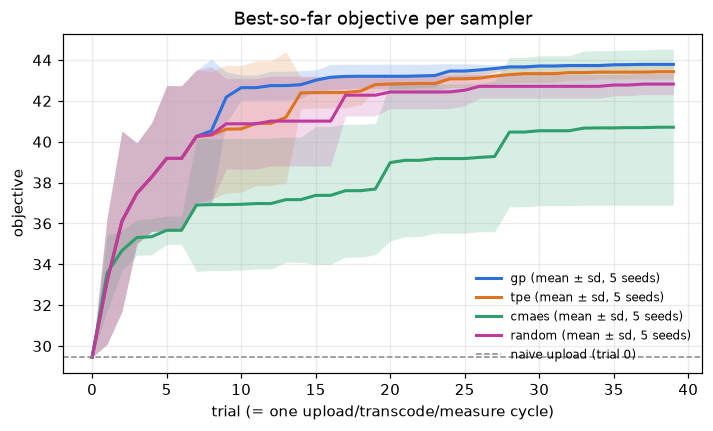
\includegraphics[width=0.75\linewidth]{p0/convergence.png}
  \caption{Best-so-far composite objective versus trial, mean and spread over five seeds per sampler
  (\texttt{ugc\_strict}).}
  \label{fig:convergence}
\end{figure}

\paragraph{Tier gain versus filter gain.}
\Cref{tab:e2} applies the decomposition of \cref{def:decomposition} and re-scores each configuration
with the judges. The tier gain ($\times2$ upload over naive) is confirmed by all three judges on all
four natural clips. The filter gain of the GP-BO configuration on \texttt{ugc\_strict} raises the
objective and both of its perceptual components on every natural clip, but it lowers SSIMULACRA2 and
XPSNR on every natural clip, and DISTS is flat. It is therefore not judge-confirmed. The same holds
for all five GP-BO seeds (0--1 of 3 judges). On \texttt{ugc\_av1} the filter gain passes the rule on
the means, but only because of one clip (park\_joy), where the AV1 tier-only upload is worse than the
naive upload on SSIMULACRA2 and the filters recover part of that loss.

\begin{table}[t]
  \centering
  \small
  \caption{Mean gain over the reference configuration on the four natural clips (park\_joy,
  old\_town\_cross, ducks\_take\_off, in\_to\_tree). The judges are SSIMULACRA2, DISTS and XPSNR;
  the last column counts judges with a positive mean gain.}
  \label{tab:e2}
  \setlength{\tabcolsep}{4pt}
  \resizebox{\linewidth}{!}{%
  \begin{tabular}{@{}lrrrrrrc@{}}
    \toprule
    Configuration (over reference) & composite & VMAF\textsubscript{NEG} & LPIPS & SSIMU2 & DISTS & XPSNR & judges \\
    \midrule
    Tier: $\times2$ over naive, \texttt{ugc\_strict} & +12.27 & +9.50 & +0.0657 & +23.02 & +0.0267 & +1.54 & 3/3 \\
    Filters: GP-BO over tier-only, \texttt{ugc\_strict} & +3.03 & +1.87 & +0.0280 & $-2.23$ & +0.0003 & $-0.75$ & 1/3 \\
    Filters: GP-BO over tier-only, \texttt{ugc\_av1} & +4.94 & +3.13 & +0.0437 & +1.90 & +0.0071 & +0.21 & 3/3$^\ast$ \\
    Learned $G$ (round 0) over tier-only & +2.55 & $-1.03$ & +0.0832 & $-5.17$ & +0.0101 & +1.24 & 2/3 \\
    \bottomrule
  \end{tabular}}\\[2pt]
  {\footnotesize $^\ast$Carried by park\_joy; on the other three natural clips SSIMULACRA2 and XPSNR are slightly lower.}
\end{table}

\paragraph{Where the filter gain comes from.}
Freezing contrast and saturation (\texttt{eq}) and re-running the search yields a sharpening-only
configuration ($\times2$, unsharp 0.89, $5\times5$, no grain). It keeps 72\,\% of the composite gain
and all of the LPIPS gain, and it passes two of three judges (DISTS $+0.0035$, XPSNR $+0.52$);
SSIMULACRA2 is still lower than tier-only ($-1.74$). The colour and contrast increase, together with
the grain that the optimiser adds alongside it, thus accounts for about 30\,\% of the composite gain
and turns XPSNR and DISTS negative. At the native tier ($\times1$, no tier change), a filter-only
search finds the same $+3.0$ composite gain almost entirely from an 11\,\% contrast increase, and no
judge agrees (0/3).

\paragraph{A Goodhart matrix.}
We optimise each of four objectives in turn and judge every result with all metrics
(\cref{fig:goodhart}). No objective is free of regressions on the metrics it does not optimise.
Optimising SSIMULACRA2 comes closest (one small regression, XPSNR $-0.24$) but gains little on its
own metric ($+0.54$). Optimising LPIPS alone saturates colour, sharpening and grain and is the worst
row on every other metric (SSIMULACRA2 $-14.9$).

\begin{figure}[t]
  \centering
  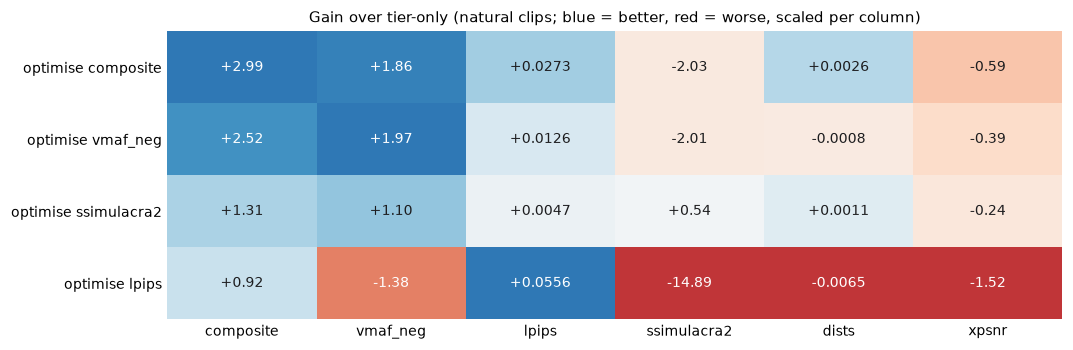
\includegraphics[width=0.8\linewidth]{p0/goodhart_matrix.png}
  \caption{Goodhart matrix. Rows: the objective optimised by GP-BO (40 trials). Columns: gain of the
  best configuration over tier-only, mean over the four natural clips, for each metric.}
  \label{fig:goodhart}
\end{figure}

\paragraph{Learned pre-compensation.}
Without a trust region ($\lambda=0$, $\delta=0.15$), the learned pre-compensation moves pixels by
18--32 levels on average; on its outputs the emulator's PSNR against the real playback falls to
19--25\,dB, and real quality collapses (old\_town\_cross: 60.4 for tier-only, 39.0 with $G$). With
the trust region, $G$ is above tier-only on the objective on three of four natural clips across
seeds (not on ducks\_take\_off), and, for seed 0, on XPSNR (4/4 clips) and DISTS (3/4); SSIMULACRA2
is lower on every clip in every seed (\cref{tab:e2}). Across seeds
(3 for $G$, 5 for the parametric configuration), $G$ beats the parametric configuration only on
old\_town\_cross and only on the objective ($65.39\pm0.87$ versus $62.62\pm0.16$); on the held-out
in\_to\_tree they tie, and the parametric configuration wins on SSIMULACRA2. $G$ damages the held-out
synthetic gradient clip far more than the parametric configuration ($-10.1$ composite over
tier-only). Domain-adaptation rounds did not improve the result.

\paragraph{Graphics and text.}
The parametric configuration found on natural clips lowers the composite of the synthetic test
pattern by 11.6 relative to tier-only, mostly through CAMBI's response to the added grain, and lowers
XPSNR by 7.0. Pre-compensation therefore has to be content-dependent, which motivates P1.

\subsection{P1: content-scoped learned pre-compensation}
\label{sec:results-p1}

\pending{E20: per-class baseline table (naive, tier-only, global sharpening-only, class-tuned
sharpening-only) on train and dev clips.}

\pending{E21: perceptual loss chosen for $G$ (LPIPS, DISTS or both) and the dev numbers behind the
choice.}

\pending{E22: global versus specialist $G$ on dev, 3 seeds; the pre-E23 decisions (the $G$ used for
class A, any additional nominated class, the gate table), with the commit in which they were frozen.}

\pending{E23: confirmation table for class A with bootstrap intervals; verdicts for H1, H2, H3; gated
system versus tier-only and the global sharpening-only configuration on all confirmation clips.}

\subsection{Real platforms}
\label{sec:results-p2}

\pending{P2 E15: measured ladder of one real platform (upload resolution and bitrate versus served
codec and bitrate), repeated uploads to measure non-determinism.}

\pending{P2 E16: real closed loop, naive versus tier-only versus sharpening-only versus the selected
configuration, with the number of uploads used.}

\pending{P2 E17: paired-comparison viewer study (tier-only versus sharpening-only versus $G$).}

\section{Discussion}
\label{sec:discussion}

\paragraph{What an uploader can gain.}
On the simulated platforms, the tier choice dominates and is confirmed by every judge. The filter
gain on top of it is small, depends on the platform, and is mostly not confirmed by metrics that were
not optimised. The only filter that survives two of three judges is plain sharpening.
\pending{update with the P1 verdict: whether a learned pre-compensation adds anything for a defined
content class, and with the real-platform results.}

\paragraph{Evaluation lessons.}
Three practices changed our conclusions and, we believe, should be standard for pre-processing work:
decomposing the gain into the tier gain and the filter gain; judging with metrics that the optimiser
never sees; and reporting variability across seeds and clips rather than single runs. Without them,
the composite results alone would have read as a consistent filter gain of about three points over
the tier trick on every natural clip.

\paragraph{Limitations.}
\begin{itemize}
  \item Most results use simulated platforms whose ladders are plausible but invented.
        \pending{state what the real-platform probe confirmed or contradicted.}
  \item Clips are 3\,s long and 720p. Natural content comes from professionally shot test
        sequences, not phone-recorded user content.
  \item Class C has a single clip, so the hypothesis about flat and dark content is untested.
        Confirmation splits contain six or seven clips per class, which limits statistical power.
  \item Retiming 24/25\,fps sources to 30\,fps speeds up their motion and raises TI.
  \item The composite objective's weights were set by hand.
  \item No metric is a substitute for viewers. \pending{viewer study.}
\end{itemize}

\section{Conclusion}
\label{sec:conclusion}

\todo{Write last, after P1 and P2. Two or three sentences: what was asked, what the evidence says,
what an uploader should do.}

\section*{Ethics and Terms of Service}
Real-platform experiments use only the authors' own accounts and content, uploaded as private or
unlisted, rate-limited, and within each platform's terms of service. The aim is better playback of
one's own content; the methods are not intended to evade moderation or to make a platform spend
additional resources. \todo{name the platform(s) and the terms that apply once P2 is run.}

\section*{Data and Code Availability}
The implementation, the clip manifest with per-clip sources and licenses, the content features,
the frozen class and split assignments, and the scripts that produce every table are available at
\todo{repository URL and the commit or release tag used for this version}. Third-party video is
not redistributed; the manifest lists where to obtain each clip.
\todo{add a LICENSE file to the repository before release.}

\section*{Use of AI Tools}
\todo{Describe which parts of the work used AI assistance (for example code, analysis scripts,
literature search, drafting) and confirm that the authors checked all results and take full
responsibility for the content. Follow arXiv's current policy and the target venue's policy.}

\section*{Acknowledgements}
\todo{Professor or others who gave feedback, compute, if any.}


\bibliographystyle{plainnat}
\bibliography{references}

\appendix
\section{Additional P0 Details}
\label{app:p0}

\paragraph{Decomposition per clip (seed 0, \texttt{ugc\_strict}, composite).}
\Cref{tab:transfer} lists the naive, tier-only and best configuration per clip. The best
configuration was found on park\_joy and old\_town\_cross; the other clips are held out.

\begin{table}[h]
  \centering
  \caption{Composite objective per clip for the naive upload, the tier-only upload ($\times2$) and the
  GP-BO configuration (seed 0). Composite only; see \cref{tab:e2} for the judges.}
  \label{tab:transfer}
  \begin{tabular}{@{}lrrrr@{}}
    \toprule
    Clip & Naive & Tier-only & Best & Filter gain \\
    \midrule
    old\_town\_cross (train) & 54.66 & 60.40 & 62.37 & +1.97 \\
    park\_joy (train)        & 4.24  & 22.21 & 25.24 & +3.03 \\
    ducks\_take\_off         & 9.39  & 25.97 & 29.37 & +3.40 \\
    in\_to\_tree             & 49.49 & 58.28 & 61.99 & +3.71 \\
    sky\_gradient (synthetic) & 92.44 & 93.07 & 93.16 & +0.09 \\
    mandelbrot (synthetic)   & $-18.98$ & $-10.22$ & $-9.38$ & +0.84 \\
    testsrc (synthetic)      & 68.26 & 69.43 & 57.87 & $-11.56$ \\
    \bottomrule
  \end{tabular}
\end{table}

\paragraph{Goodhart matrix (numbers).}
Gains over tier-only, mean over the four natural clips; bold cells are optimised by the row's
objective (the composite contains VMAF NEG and LPIPS).

\begin{table}[h]
  \centering
  \small
  \caption{Numbers behind \cref{fig:goodhart}.}
  \label{tab:goodhart}
  \begin{tabular}{@{}lrrrrrr@{}}
    \toprule
    Objective & composite & VMAF\textsubscript{NEG} & LPIPS & SSIMU2 & DISTS & XPSNR \\
    \midrule
    composite   & \textbf{+2.99} & \textbf{+1.86} & \textbf{+0.0273} & $-2.03$ & +0.0026 & $-0.59$ \\
    VMAF NEG    & +2.52 & \textbf{+1.97} & +0.0126 & $-2.01$ & $-0.0008$ & $-0.39$ \\
    SSIMULACRA2 & +1.31 & +1.10 & +0.0047 & \textbf{+0.54} & +0.0011 & $-0.24$ \\
    LPIPS       & +0.92 & $-1.38$ & \textbf{+0.0556} & $-14.89$ & $-0.0065$ & $-1.52$ \\
    \bottomrule
  \end{tabular}
\end{table}

\paragraph{Learned pre-compensation versus the parametric configuration across seeds.}

\begin{table}[h]
  \centering
  \small
  \caption{Composite and SSIMULACRA2 per clip, mean $\pm$ sd over seeds ($G$: 3 seeds, round 0;
  GP-BO configuration: 5 seeds).}
  \label{tab:g-vs-theta}
  \setlength{\tabcolsep}{4pt}
  \begin{tabular}{@{}lrrrrr@{}}
    \toprule
    & & \multicolumn{2}{c}{composite} & \multicolumn{2}{c}{SSIMULACRA2} \\
    \cmidrule(lr){3-4}\cmidrule(lr){5-6}
    Clip & Tier-only & GP-BO & $G$ & GP-BO & $G$ \\
    \midrule
    park\_joy (train)          & 22.21 & $24.95\pm0.17$ & $22.75\pm0.21$ & $-23.57\pm0.94$ & $-27.11\pm0.46$ \\
    old\_town\_cross (train)   & 60.40 & $62.62\pm0.16$ & $65.39\pm0.87$ & $51.48\pm0.78$ & $50.87\pm0.96$ \\
    ducks\_take\_off (train for $G$) & 25.97 & $29.09\pm0.27$ & $25.45\pm0.38$ & $-23.29\pm1.10$ & $-26.99\pm0.98$ \\
    in\_to\_tree (held out)    & 58.28 & $62.59\pm0.40$ & $62.32\pm0.81$ & $42.73\pm0.66$ & $38.31\pm1.54$ \\
    sky\_gradient (held out)   & 93.07 & $92.87\pm0.29$ & $82.99\pm1.56$ & $86.18\pm0.95$ & $66.91\pm4.47$ \\
    \bottomrule
  \end{tabular}
\end{table}


\end{document}
